\newpage
\section{Modellazione AMS}

Il sistema è composto da una tanica d'acqua, dalla valvola che regola l'apertura della tanica e dal proprio controllore.

\begin{figure}[htbp]
    \centering
    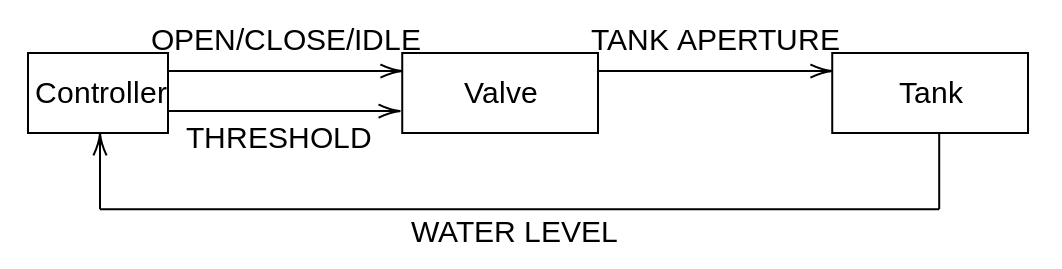
\includegraphics[width=0.5\textwidth]{schemi/ams-tank-valve.png}
    \caption{Schema del sistema tanica d'acqua}
    \label{fig:ams-tank-valve}
\end{figure}

La tanica mantiene al suo interno l'acqua. Il livello di riempimento è dato dalla funzione $x(t)$. Occorre che $5.0 \le x(t) \le 8.8$. Il livello di riempimento è dato dal sistema
\[ \begin{cases}
    \dot{x} = 0.6 a - 0.03 x \\
    x(0) = 0 
\end{cases} \]

La valvola aggiorna il livello proprio livello di apertura $a$ a seconda del comando che riceve dal controllore. I valori esatti sono presenti in Tabella~\ref{tab:ams-comandi}. In ogni caso occorre che $0 \le a(t) \le T$ con $T$ threshold in input dal controllore. Il valore iniziale si suppone sia $a(0) = 0$.

Il controllore monitore il livello dell'acqua e comanda la valvola di conseguenza. I comandi generati sono \code{OPEN}, \code{IDLE} e \code{CLOSE}. Un threshold (inteso come valore massimo) viene aggiornato secondo i valori di Tabella~\ref{tab:ams-comandi} e mandato alla valvola. Il suo valore iniziale è $T(0) = 0.7$.

\begin{table}[htbp]
    \centering
        \begin{tabular}{lrrrr}
        Segnale & Min lev & Max lev & Molt. threshold & Molt. $a$ \\ \hline
        \code{OPEN} & 0.0 & 5.0       & 1.1x &  0.25x \\
        \code{IDLE} & 5.0 & 8.8       & 1.0x &  0.00x \\
        \code{CLOSE} & 8.8 & $\infty$ & 0.7x & -0.25x
    \end{tabular}
    \caption{Comandi dati dal controllore alla valvola, range di livello di acqua del comando, moltiplicatore per l'aggiornamento del threshold, moltiplicatore per l'aggiornamento del livello di apertura}
    \label{tab:ams-comandi}
\end{table}

\subsection{Valvola}

La valvola è implementata tramite il modello discreto non conservativo AMS-TDF. Il suo compito è aggiornare il valore dell'apertura a seconda del comando ricevuto. La classe è definita tramite la macro \code{SCA\_TDF\_MODULE} e tutta la logica del componente è racchiusa nel metodo \code{processing}.

\subsection{Controllore}

Il controllore è implementato tramite il modello discreto non conservativo AMS-TDF. Il suo compito è ricevere il livello dell'acqua dal serbatoio e generare i comandi ed il threshold da passare alla valvola. a classe è definita tramite la macro \code{SCA\_TDF\_MODULE} e tutta la logica del componente è racchiusa nel metodo \code{processing}. Viene settato un ritardo obbligatorio sulla porta in input per poter definire un ordine di esecuzione per i componenti (scheduling). Il ritardo viene settato nel metodo \code{set\_attributes}. 

\subsection{Serbatoio}

Il serbatoio è implementato tramite AMS-LSF (a tempo continuo, non conservativo). 
\begin{figure}[htbp]
    \centering
    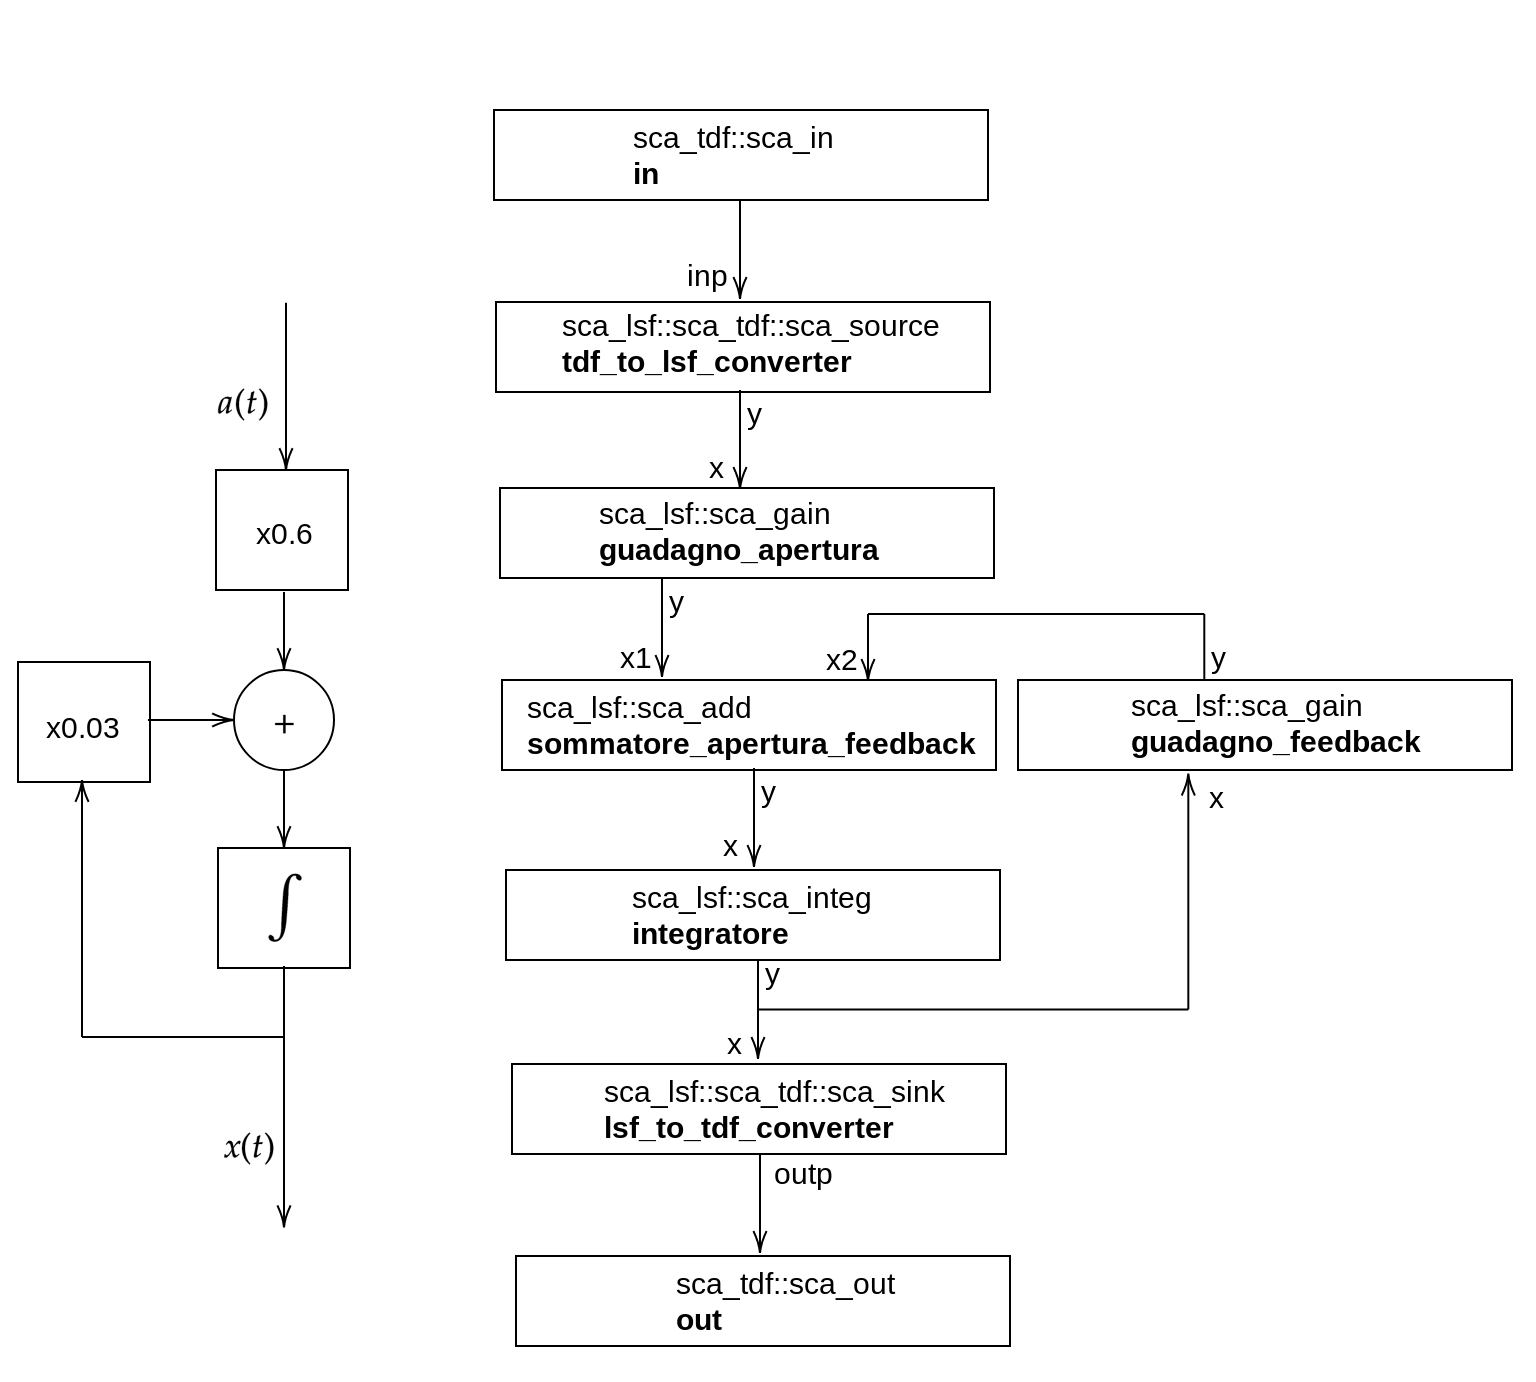
\includegraphics[width=0.5\textwidth]{schemi/ams-water-tank.png}
    \caption{Serbatoio. A sinistra lo schema ad alto livello, a destra lo schema con i componenti LSF. Per ogni blocco, la prima riga nel rettangolo è il tipo del componente, la seconda riga il nome, le etichette vicino alle frecce i nomi delle porte del componente.}
    \label{fig:ams-tank}
\end{figure}
Poichè il resto del sistema è a tempo discreto abbiamo due elementi che convertono il segnale TDF in LSF continuo e viceversa. I componenti utilizzati sono visibili in Figura~\ref{fig:ams-tank}.

\subsection{Risultato}

Vediamo di seguito che dopo diverse oscillazioni il livello dell'acqua si stabilizza ad $8.507$.
\begin{center}
    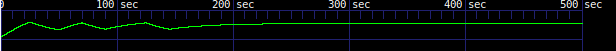
\includegraphics[width=0.5\textwidth]{schemi/ams-esito.png}
\end{center}